%!TEX root = ../../super_main.tex

\section{Automated Testing}
\label{sec:automated_unit_test}

Our development method states that all code we develop should be made in a test-first fashion (see \secref{sec:extreme_programming}). We therefore attempted to always make test cases for all the features we implemented. Our code coverage graphs can be seen in \figref{fig:android_project_code_coverage} and \figref{fig:php_project_code_coverage}, for our Android and PHP projects respectively. The two figures look different because we use different plugins on the CI server (due to the projects being written in different languages). We have not used a more strict testing metric than line coverage, due to limited time. However, interesting and useful metrics might include branch coverage, exception handling, etc. This does not mean that we did not write test cases which tests for correct exception handling, we simply did not have any automated way of calculating metrics for it. In the Android project our line coverage percentage is $\sim 43\%$, which is relatively low. %But as explained previously, this is due to the complexity of the integration tests which were manual instead. 

% In \figref{fig:android_project_code_coverage} the line coverage is represented with green while missed lines are represented with red. In \figref{fig:php_project_code_coverage} the red line is method coverage, blue is line coverage and green is total.

\begin{figure}[!htbp]
    \centering
    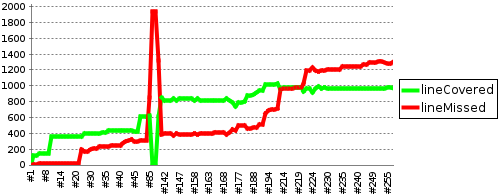
\includegraphics[width=0.7\textwidth]{graphic/quality_assurance/jenkins_android_code_coverage}
    \caption{Android project code coverage}
    \label{fig:android_project_code_coverage}
\end{figure}
\FloatBarrier

In the PHP project, we have a $\sim 74\%$ line coverage, which is rather good. Most of the untested code is library- or auto generated code, and we have not tested this because we assume these parts work as they are supposed to. This is a risk management assessment we have made, and deemed insignificant, in contrast to the speed we gain from using the libraries without testing them. % If we only considered coverage on the code we made ourselves, it would probably exceed 90\%. 

\begin{figure}[!htbp]
    \centering
    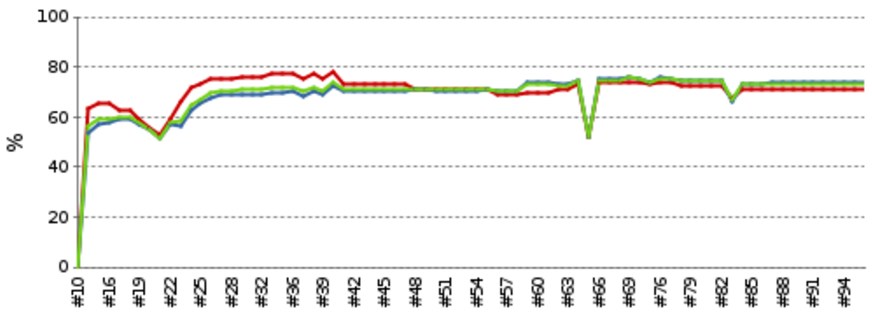
\includegraphics[width=0.7\textwidth]{graphic/quality_assurance/jenkins_php_code_coverage}
    \caption{PHP project code coverage}
    \label{fig:php_project_code_coverage}
\end{figure}
\FloatBarrier

\subsection{Manual Test}
In some cases it was not possible to, in decent time, create automatic dynamic white box tests, and we therefore, in these cases, switched to a dynamic black box approach instead. Here we made test specifications, executed some part of the code manually and observed the result relative to the specifications. We mainly did this for the more complex parts of the code, such as the \mono{BackgroundSensorService} class, which schedules all the \mono{SensorProvider}s asynchronously and sends the results to the server. Here we test if the sensor provider outputs the data correctly to the server. We also used this approach for other testing methods, such as integration testing. For instance, we would, when a new UI-related feature was implemented, manually test if previous UI features would still work. We did not spend time on specifying written test-cases on the most basic integration tests, such as ``is it possible to subscribe to a campaign?'', since these would probably be found during ad-hoc testing done while developing new features.
\\\\
These manual tests resulted in a generally lower line coverage, especially on the Android project, since the CI plugin we used was unable to compare our manual tests to the code base. This does not necessarily mean that the code is less tested, but it is harder to tell when tests are covering the code base well. 